% preamble and style file for M&R lecture slides
\documentclass[11.5pt,sans,english]{beamer}

\usetheme{EastLansing}
\usecolortheme{lily}

\usepackage[most]{tcolorbox}

\usepackage{verbatim}
%\usepackage{ulem}
%\usepackage{fontawesome}
%\usepackage{tikz}
%\usepackage{pifont}
%\usepackage{tabularx}
\usepackage{array,booktabs,xcolor,colortbl,multirow,rotating,amssymb}
%\usepackage{amsmath}
% \usepackage{vwcol}
% \usepackage[T1]{fontenc}

  
\newcommand\vect[1]{\underline{\mathbf{#1}}}
\newcommand\unitvect[1]{\hat{\boldsymbol{#1}}}
%\newcommand\hatdot[1] { \hat{ \dot{ \boldsymbol{#1} } } }

\newtcbox
{\keyc}{on line,arc=2pt, colback=yellow!30!white, colframe=yellow!30!black, before upper={\rule[-3pt]{0pt}{10pt} },boxrule=1pt,boxsep=0pt,left=6pt,right=6pt,top=2pt,bottom=2pt,}

\newtcbox
{\keyb}{on line,arc=1pt, colback=blue!30!white, colframe=blue!30!black, before upper={\rule[-3pt]{0pt}{10pt} },boxrule=1pt,boxsep=0pt,left=6pt,right=6pt,top=2pt,bottom=2pt,}

\newtcbox
{\keyl}{on line,arc=1pt, colback=pink!30!white, colframe=blue!30!black, before upper={\rule[-3pt]{0pt}{10pt} },boxrule=1pt,boxsep=0pt,left=6pt,right=6pt,top=2pt,bottom=2pt,}

\newtcbox
{\keyw}{on line,arc=1pt, colback=red!30!white, colframe=blue!30!black, before upper={\rule[-3pt]{0pt}{10pt} },boxrule=1pt,boxsep=0pt,left=6pt,right=6pt,top=2pt,bottom=2pt,}

\newtcbox
{\keya}{on line,arc=1pt, colback=purple!30!white, colframe=blue!30!black, before upper={\rule[-3pt]{0pt}{10pt} },boxrule=1pt,boxsep=0pt,left=6pt,right=6pt,top=2pt,bottom=2pt,}

\newtcbox[auto counter,number within=section]
{keyf}
{
enhanced,
on line,
  boxsep=0pt,
  left=6pt,right=6pt,top=2pt,bottom=2pt,
  arc=5pt,
  boxrule=1pt,
  rightrule=38pt,
colback=green!10!white, 
colframe=green!50!black, 
title=\thetcbcounter,
detach title,
overlay unbroken and first ={
    \node[%rotate=90,
          %minimum width=1cm,
          anchor=south,
          font=\sffamily\bfseries\tiny,
          %yshift=-10pt,
          yshift=-5pt,
          xshift=-20pt,
          white]
    at (frame.east) {\thetcbcounter};
  }
}


\usepackage{xcolor}

%\usepackage{hyperref}
%\hypersetup{
%  pdfauthor={Lily Asquith},
%  urlcolor=blue,
%  colorlinks=true,
%  linkcolor=blue,
%  bookmarks=true
%}

%---------------------------------------------%
%              LILY'S COLOURS           %
%---------------------------------------------%
\definecolor{Wash}{RGB}{204,204,204}
%\definecolor{Pinky}{RGB}{254,200,254}%violet
\definecolor{Pinky}{RGB}{219,	240,	253}%violet
\definecolor{Bluey}{RGB}{0,190,255}%deep sky blue
\definecolor{DarkGrey}{RGB}{28,66,137}%dar grey
\definecolor{SussexWhite}{RGB}{253,255,254}%dar grey
\definecolor{LightGray}{RGB}{184,184,255}
\definecolor{YesGreen}{RGB}{0,128,0}
\definecolor{NoRed}{RGB}{250,0,0}



\definecolor{myred}{RGB}{255,153,153}
\definecolor{myorange}{RGB}{255,204,153}
\definecolor{myyellow}{RGB}{255,255,153}
\definecolor{mygreen}{RGB}{153,255,153}
\definecolor{mycyan}{RGB}{153,255,255}
\definecolor{myblue}{RGB}{153,204,255}
\definecolor{myviolet}{RGB}{153,153,255}
\definecolor{mypurple}{RGB}{204,153,255}
\definecolor{mypink}{RGB}{255,204,255}
\definecolor{mycoral}{RGB}{255,153,204}

%-----------------------------------------------------%
%              LILY'S COLUMN TYPES          %
%-----------------------------------------------------%
\newcolumntype{a}{>{\raggedright\arraybackslash}l}	
\newcolumntype{q}{>{\raggedright\arraybackslash}m{8cm}} 

%--------------------------------------------%
%              LILY'S SYMBOLS          %
%--------------------------------------------%
\newcommand{\dfinger}{\large{\textcolor{black}{\ding{43}}}\scriptsize}
\newcommand{\dstar}{\large{\textcolor{black}{\ding{76}}}\scriptsize}
\newcommand{\dwrite}{\large{\textcolor{black}{\ding{45}}}\scriptsize}
\newcommand{\ddiamond}{\small{\textcolor{DarkGrey}{\ding{117}}}\scriptsize}
\newcommand{\ddiamondwhite}{\small{\textcolor{SussexWhite}{\ding{117}}}\scriptsize}
\newcommand{\experiment}{\small{\textcolor{magenta}{\faCogs }}\scriptsize}
\newcommand{\watchit}{\textcolor{blue}{ \faYoutube}}


\makeatletter
\newcommand\notsotiny{\@setfontsize\notsotiny{6.5}{7.5}}
\makeatother


% 
\title[ Intro to Quantum Physics]{Intro to Quantum Physics F3241}
%\subtitle{\textbf{Part 1: Preface}}
\author[Dr Lily Asquith (Lily)]{ Dr Lily Asquith (Lily)}
\date[27 Sep - 01 Oct 2021]{ 27 Sep - 01 Oct 2021 (Week 1)}
\logo{

\includegraphics[width=1cm]{../../utils/uslogo.jpg}
}


\begin{document}


\begin{frame}
\titlepage
\end{frame} 

 %-----------------------------------------------------------%
 % 1 Kinematics                                                 %
 %-----------------------------------------------------------%
\section{I2Q Part 1: Preface}
\begin{frame}
\frametitle{Preface} 
\normalsize

This week's topics:\\[3ex]

\begin{itemize}
\item[1.1] Units, prefixes, and dimensionality\\[3ex]
\item[1.2] Constants\\[3ex]
\item[1.3] Tips \& Tricks\\[3ex]
\end{itemize}

Your homework questions for this week are on canvas - please complete these by the end of the week.
\end{frame} 
 
 %-----------------------------------------------------------%
 % LECTURE 1
 %-----------------------------------------------------------%
 
 \subsection{Units, prefixes, and dimensionality}

\begin{frame}{Topic 1.1 : Units, prefixes, and dimensionality}
\small
\textbf{Aim:}\\
To prepare your minds for the strange things to come, by convincing you that things are already strange.\\[3ex]
\textbf{Method:}\\
We will think about how we measure the world around us now, and what led us to use these measurement techniques.\\[1ex]

\end{frame}


%  
\begin{frame}{Where did all this start?}
\small
To do physics, we need clear, agreed-upon definitions and systems of measurements.\\[1ex]
But, human beings started to do science before there was any such clarity...\\[1ex]
\begin{center}
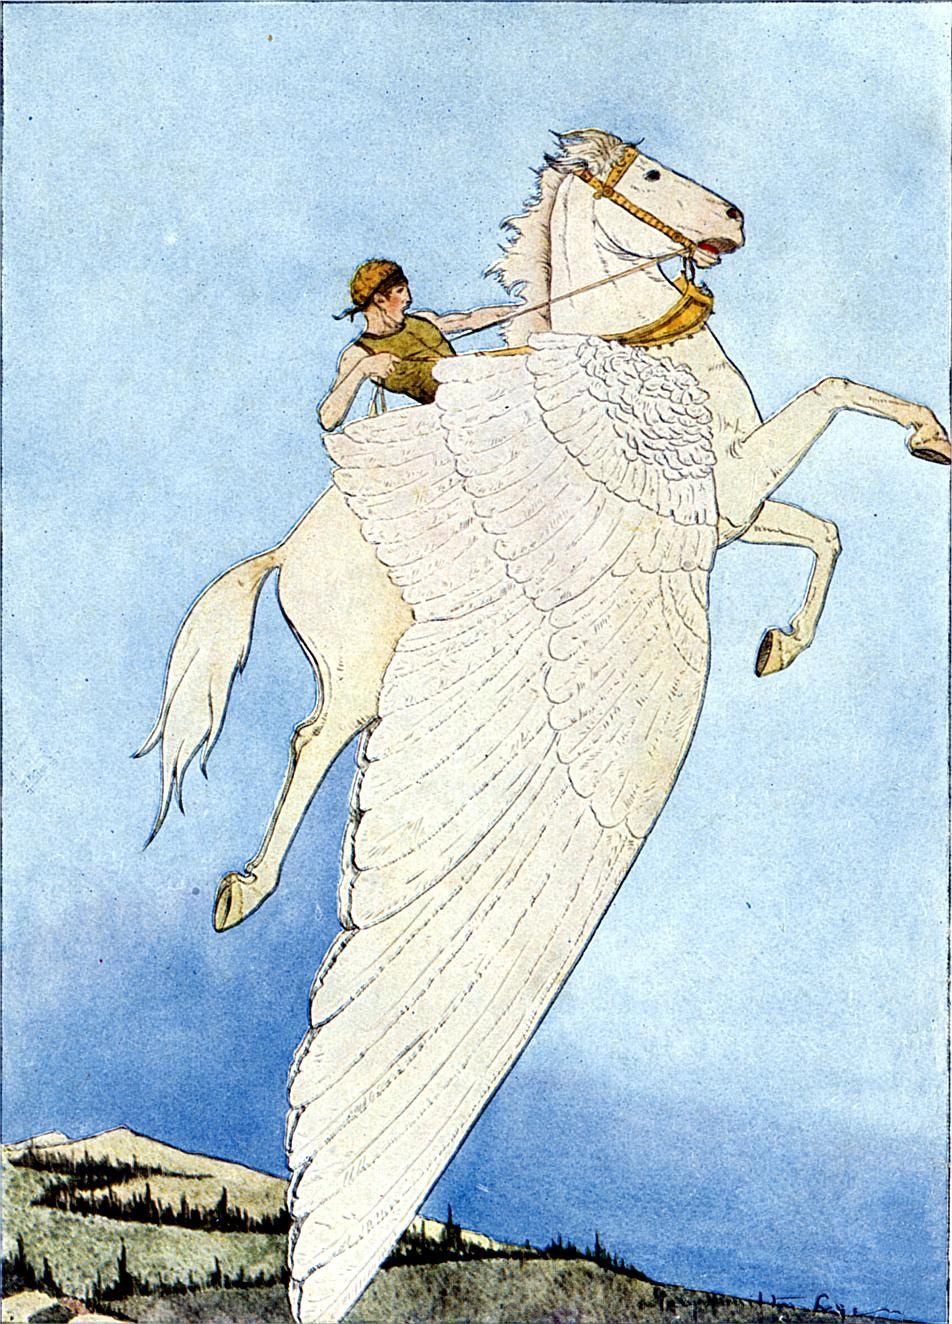
\includegraphics[scale=0.75]{pegasus.jpg}
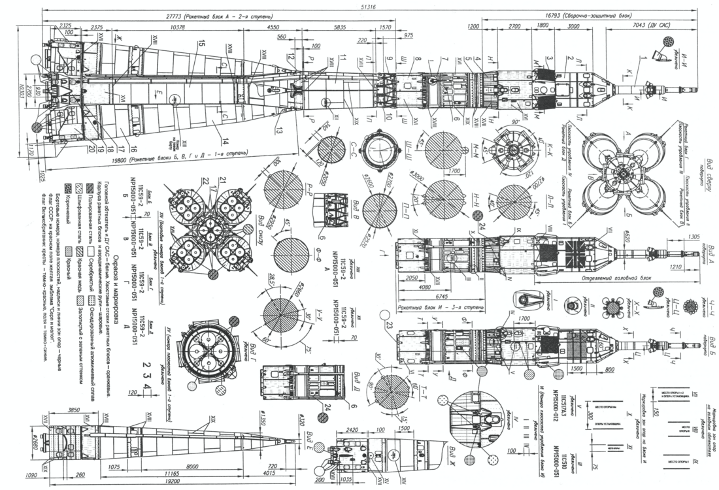
\includegraphics[scale=0.25]{absolutes.png}
\end{center}
\end{frame}

\begin{frame}{Length}
Measurements of length or distance tend to have roots in human body parts (and later, farming).\\
\begin{center}
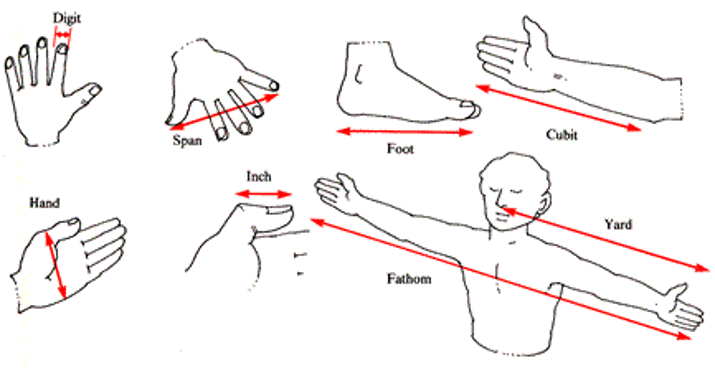
\includegraphics[scale=0.2]{length.png}
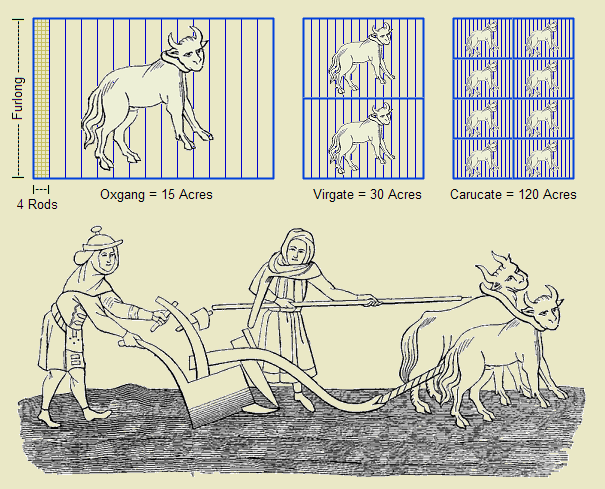
\includegraphics[scale=0.2]{humancow.png}
\end{center}
\end{frame}


\begin{frame}{Time}
Measurements of time tend to have their roots in the things we observe in the sky.\\

\begin{center}
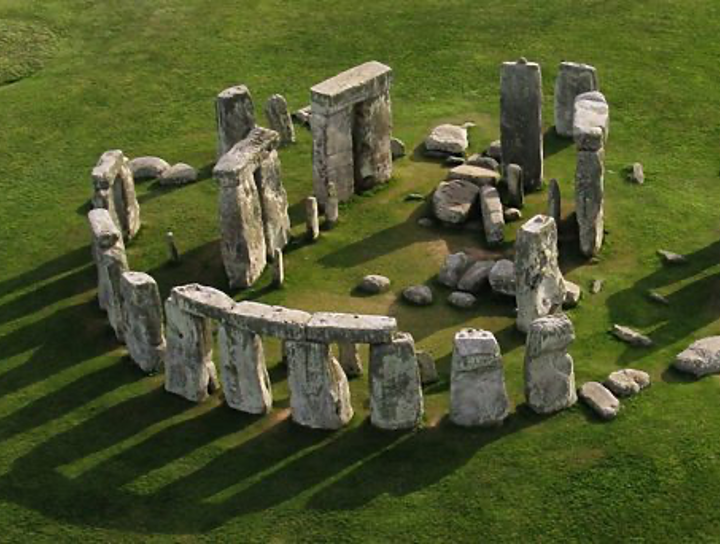
\includegraphics[scale=0.3]{time.png}
\end{center}
\end{frame}


\begin{frame}{Weight}
Measurements of weight tend to have their roots in things we can pick up.\\
\begin{center}
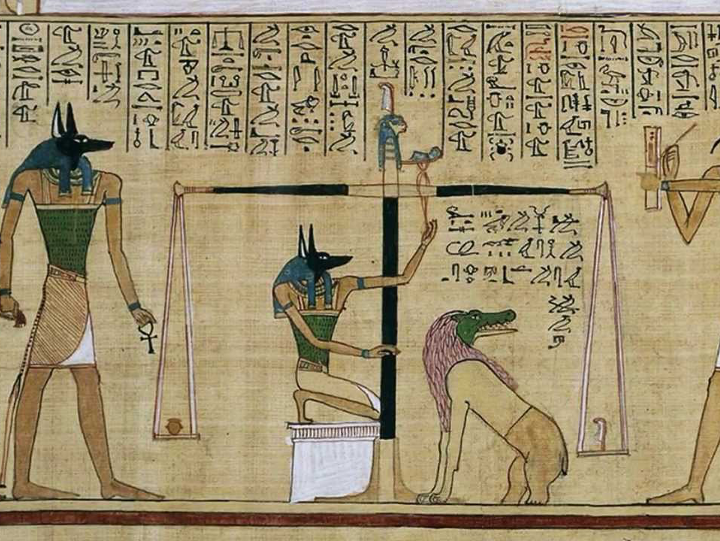
\includegraphics[scale=0.3]{weight.png}
\end{center}
\end{frame}

\begin{frame}{Units}
Thankfully, we now have the Syst\`eme International, with 7 base units: \\[1ex]
%\begin{columns}
%\begin{column}{0.5\textwidth}
\begin{itemize}
\item Metres, m\\ % The metre is currently defined as the length of the path travelled by light in a vacuum in 1/299 792 458 of a second. 
\item Seconds, s\\
\item Kilograms, kg\\ % lump of metal in parisien basement - > now defined in terms of fundamental constants

\item Amperes, A\\ %The ampere is defined by taking the fixed numerical value of the elementary charge e to be 1.602 176 634 � 10?19 when expressed in the unit C, which is equal to A?s, where the second is defined in terms of ??Cs, the unperturbed ground state hyperfine transition frequency of the caesium-133 atom
\item Kelvin, K\\ % The kelvin is now defined by fixing the numerical value of the Boltzmann constant k to 1.380649�10?23 J?K?1. Hence, one kelvin is equal to a change in the thermodynamic temperature T that results in a change of thermal energy kT by 1.380649�10?23 J.[1] The relation between kelvin and Celsius scales is TK = t�C + 273.15. On the Kelvin scale, pure water freezes at 273.15 K, and it boils at 373.15 K in 1 atm.  Absolute zero does not exist. https://www.sciencealert.com/after-a-century-of-debate-cooling-to-absolute-zero-has-been-declared-mathematically-impossible

\item Candela, cd\\
\item Mole, mol\\

\end{itemize}
%\end{column}
%\begin{column}{0.5\textwidth}
%\begin{center}
%\includegraphics[scale=0.45]{oldSI.png}
%\includegraphics[scale=0.45]{newSI.png}
%\end{center}
%\end{column}
%\end{columns}

%\tiny
%Figures: By Emilio Pisanty - Own work, CC BY-SA 4.0
\end{frame}



\begin{frame}{Lingering Issues}
\small
For some folks, the metric system has been hard to adopt.\\
\begin{center}
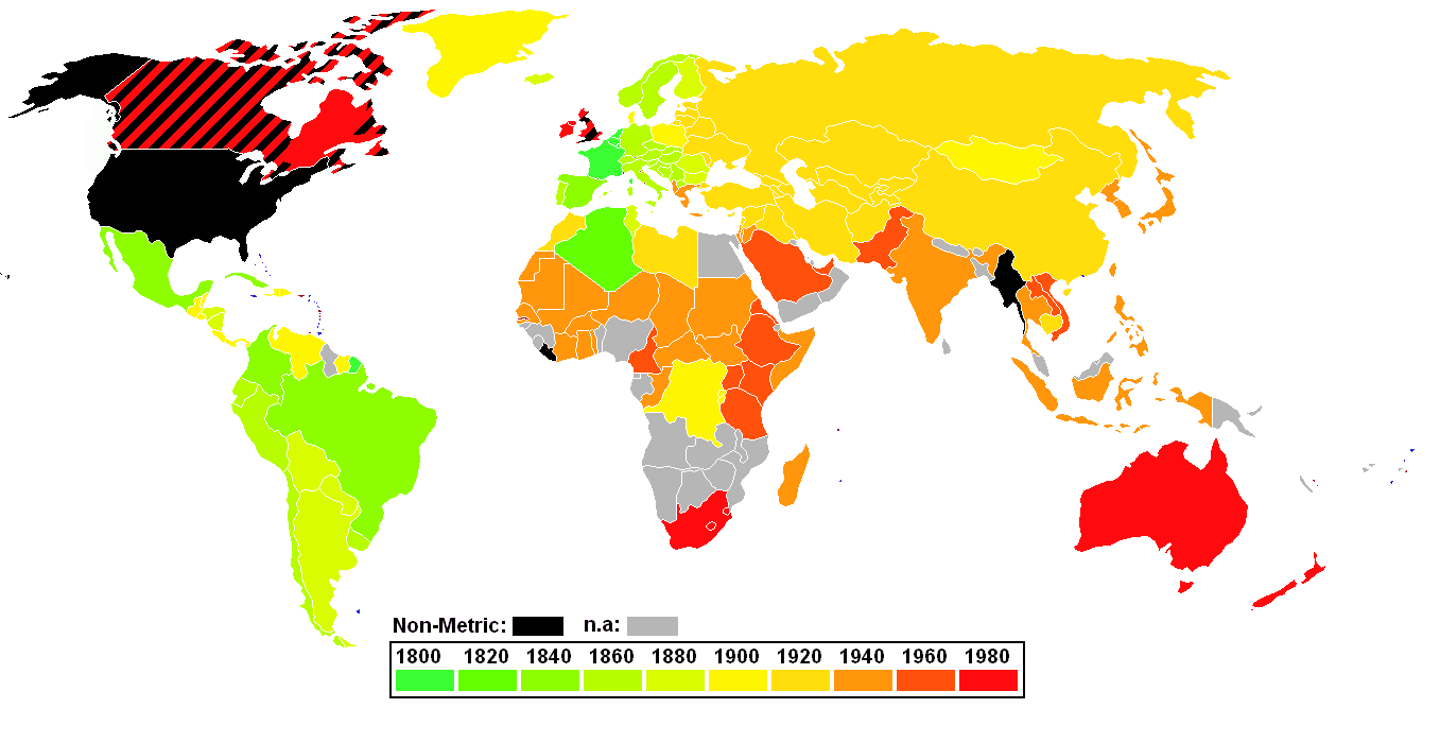
\includegraphics[scale=0.45]{metric_map.png}
\end{center}
\end{frame}





\begin{frame}{Lingering Issues}
\begin{center}

\includegraphics[scale=0.45]{uk-pint.png}

\includegraphics[scale=0.45]{us-pint.png}
\end{center}
\small
\begin{itemize}
\item 12 inches in a foot, 3 feet in a yard, 1760 yards in a mile. By the way, a mile is 8 furlongs. A fathom is 2 yards and a league is 3 miles. 
\item British pint 568 ml : 20 imperial fluid ounces, \textcolor{red}{ American pint 473 ml : 16 US ounces}
\item British Ton 2,240 pounds (20 hundredweight each of 8 stone each of 14 pounds). \textcolor{red}{American Ton 2,000 pounds}. \textcolor{blue}{Metric tonne 2204.62 pounds}
\end{itemize}

\end{frame}



\begin{frame}{Lingering Issues}
\begin{center}
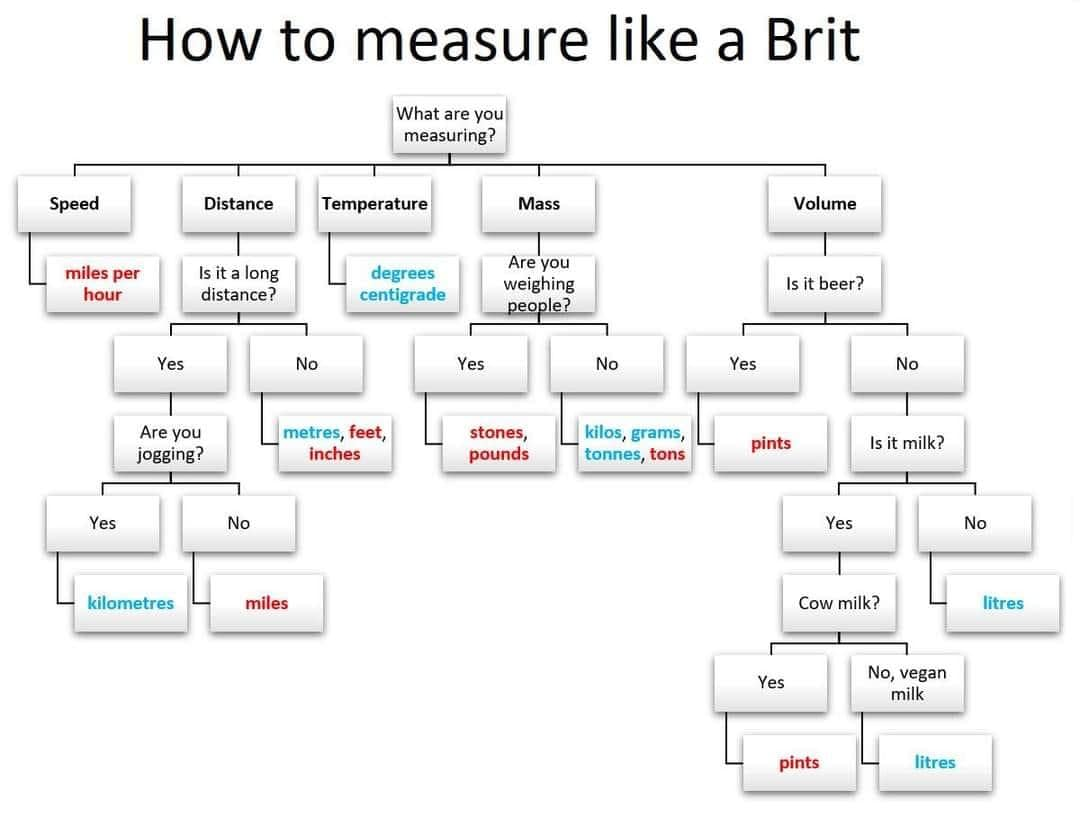
\includegraphics[scale=0.25]{measure-like-a-brit.jpg}
\end{center}
\end{frame}

%\begin{frame}{Poll everywhere checkpoint }
%
%Which is longer: a fathom, a furlong, or a mile?\\[1ex]
%
%\fbox{\begin{minipage}{\textwidth}
%Use your phone to go to: \textcolor{blue}{pollev.com/ilovephysics}
%
%\end{minipage}}
%\vspace{2cm}
%  \end{frame}


%\begin{frame}{Amounts of things}
%At some point, human beings took the step of \textbf{quantifying} things. \\[1ex]
%
%\end{frame}



\begin{frame}{Counting Systems}
\small
Like with units, the choice is based on `common sense' rather than anything fundamental:\\
\begin{itemize}
\item Sexagesimal [60]
%\item Vigesimal [20]
\item Duodecimal [12] 
\item Decimal [10]
\item Hexadecimal [16]
\item Binary [2]
\end{itemize}

\textit{Are there an infinity of possible counting systems?}
\end{frame}

\begin{frame}{Length: standardising the metre}
\small
First the pendulum was used; then, a fraction of the estimated circumference of the Earth.\\
1791 (-1799): The French National Assembly accepts the proposal that the new definition for the metre be equal to `\textit{one ten-millionth of the length of a quadrant along the Earth's meridian through Paris}'  (the distance from the equator to the north pole.)
\begin{center}
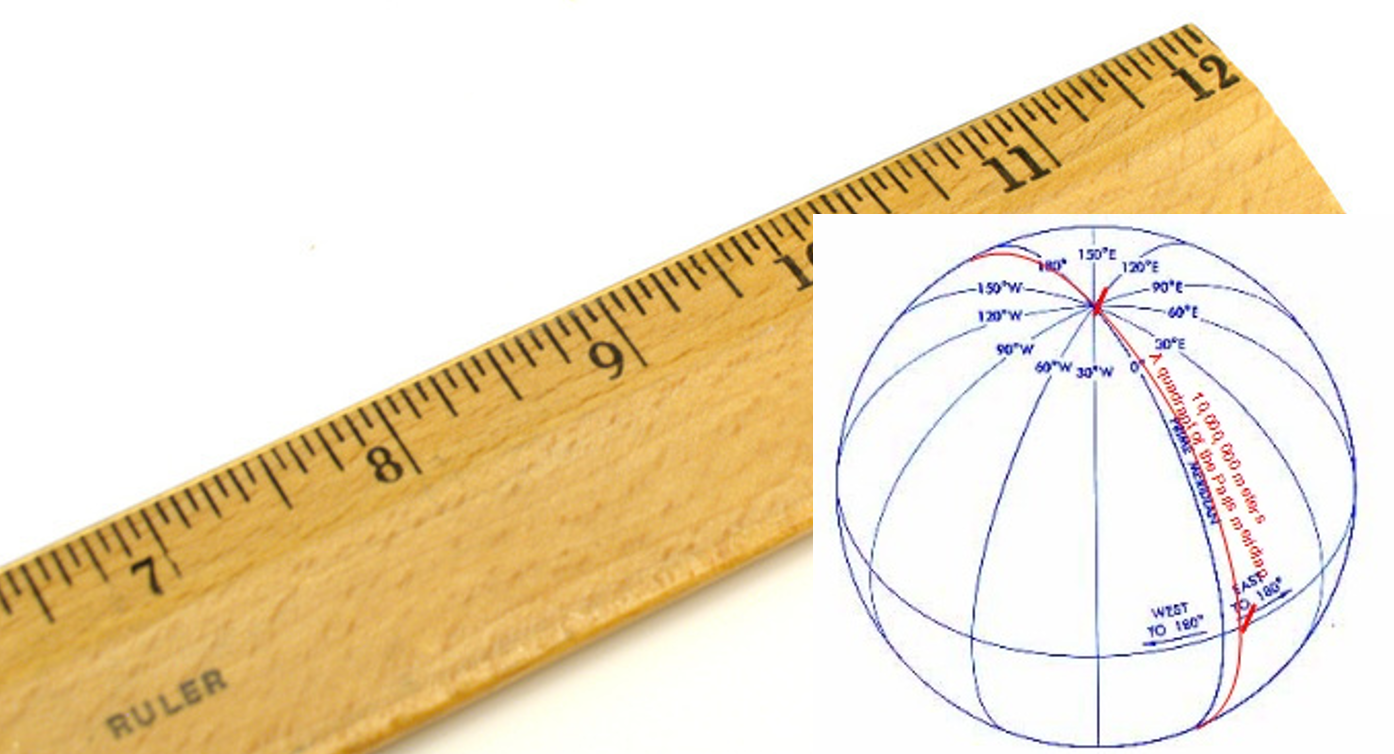
\includegraphics[scale=0.3]{metre.png}
\end{center}
\end{frame}

\begin{frame}{Time: standardising the second}
\begin{columns}
\begin{column}{0.65\textwidth}
\small
Up to 1400 CE: The earliest mechanical clocks had hours, sometimes divided into quarters, more rarely into 12 parts.\\[1ex]
Clocks with minutes appeared late 16th century, followed by seconds in 17th-18th centuries\\[1ex]
1862: The British Association for the Advancement of Science stated that `\textit{All [people] of science are agreed to use the second of mean solar time as the unit of time.}'
\end{column}
\begin{column}{0.35\textwidth}
\begin{center}
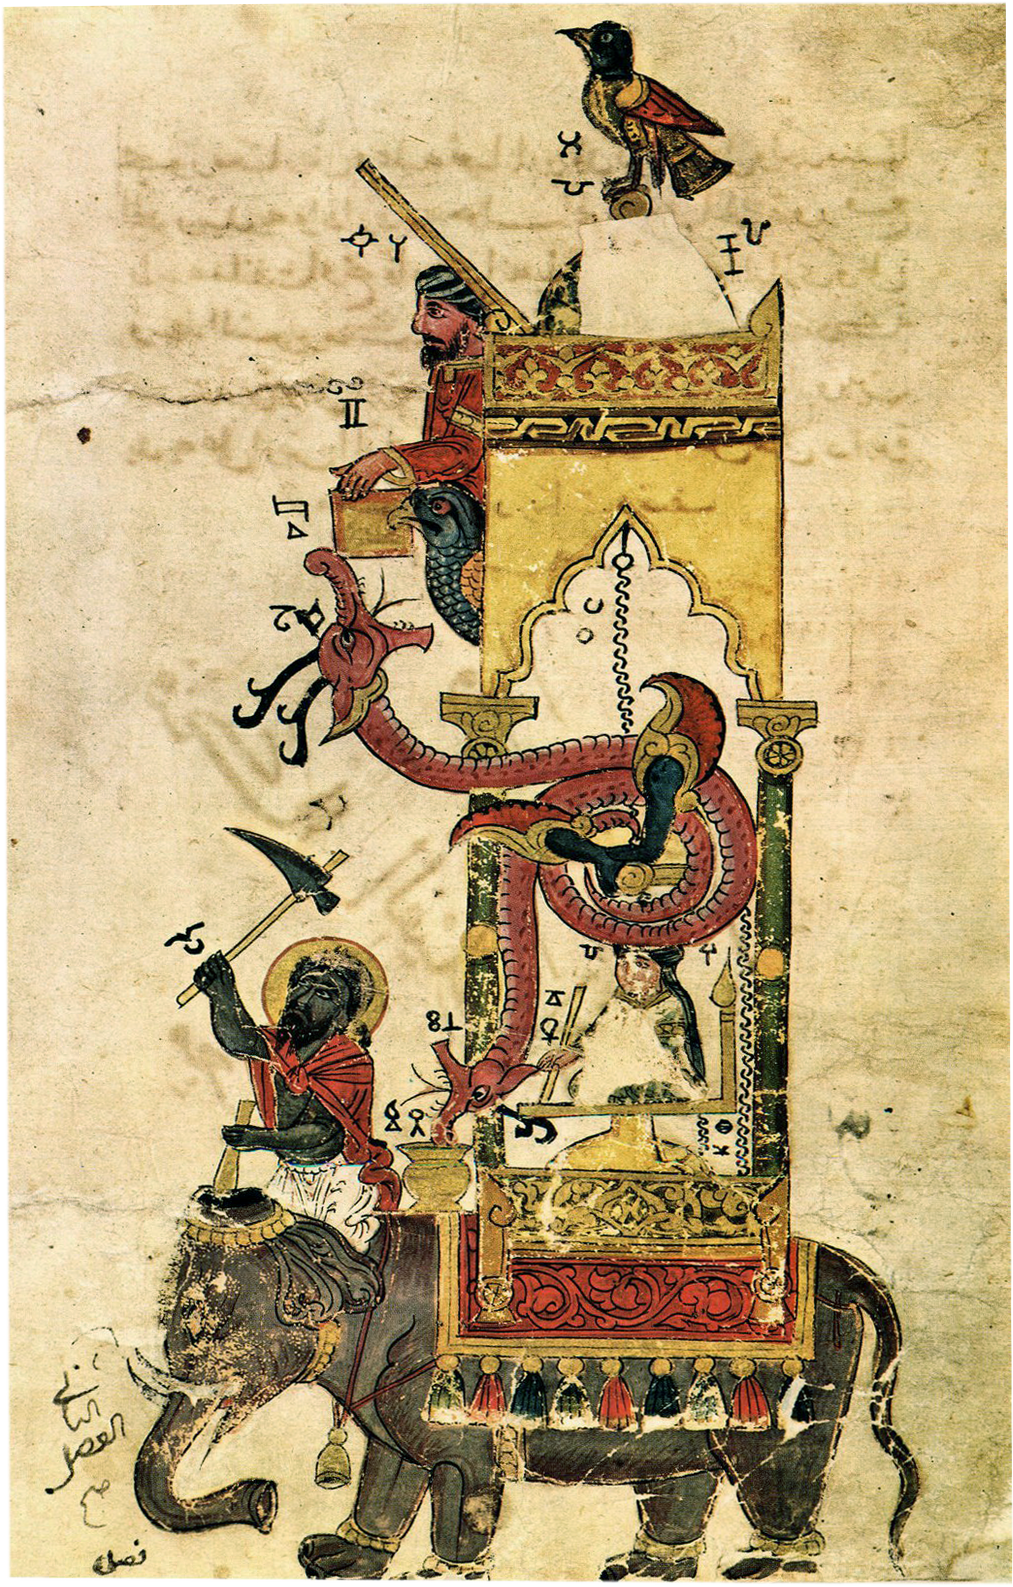
\includegraphics[scale=0.35]{elephant_clock.png}
\end{center}
\end{column}
\end{columns}
\end{frame}

\begin{frame}{Weight: standardising the kilogram}
\small
1795: the mass of 1 litre of water (at melting point).\\
There is a prototype kilogram in the custody of the International Bureau of Weights and Measures in Sevres, France. 
\begin{center}
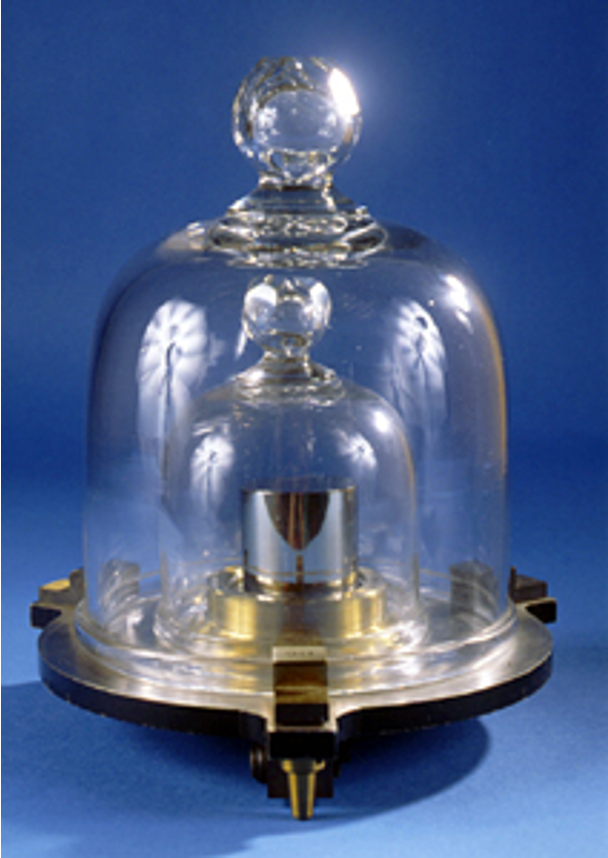
\includegraphics[scale=0.3]{kilo.png}
\end{center}
\end{frame}



 
 \begin{frame}{Er, what has this got do with quantum physics? }

The measures and counting systems we use are arbitrary, and have developed organically in a pretty chaotic way.\\[1ex]

There is nothing fundamentally meaningful about a 1 metre distance, or the number 10.\\[1ex]

We can and will abandon standard measures and units in order to make calculations easier.\\[1ex]

There are things in this universe that do seem to be fundamentally meaningful.\\[1ex]

  \end{frame}


\begin{frame}{Prefixes}
\scriptsize
%\begin{center}
\begin{tabular}{c c c l}
\textbf{Prefix} &  \textbf{Symbol} & \textbf{Factor} & \textbf{Etymology}\\[1ex]
peta & P & $10^{15}$ & Greek: `five' \\[1ex] % DATA!
tera & T & $10^{12}$ & Greek: `monster' \\ [1ex]% LHC energies
giga & G & $10^9$ & Greek: `giant' \\ [1ex]% Particle masses
mega & M & $10^6$ & Greek: `big' \\[1ex]
kilo & k & $10^3$ & Greek: `thousand' \\[2ex]

zero &  & $10^{0}$ &  Arabic: `sifr : empty'  \\[2ex]

milli & m & $10^{-3}$ &  	Latin: `thousandth' \\[1ex]
micro & $\mu$ & $10^{-6}$ &  Greek: `small' \\[1ex]
nano & n & $10^{-9}$ &  	Greek: `dwarf' \\ [1ex]% wavelengths
pico & p & $10^{-12}$ &  	Spanish: `tiny bit'\\[1ex]
femto & f & $10^{-15}$ &  	Dano-Norwegian: `fifteen'\\ [1ex]% interaction cross sections

\end{tabular}
%\end{center}

\end{frame}



 \begin{frame}{Dimensionality : LMT}
To get a grip and do useful science, we should think about what it is important.\\
\begin{itemize}
\item Length [L]\\
\item Mass [M]\\
\item Time [T]\
\end{itemize}

The dimension of area is $L^2$. \\[1ex]
\begin{itemize}
\item[a] What is the dimension of volume?\\[1ex]
\item[b] What is the dimension of density (mass/volume)?\\[1ex]
\item[c] What is the dimension of acceleration?\\[1ex]
\item[d] What is the dimension of force?\\[1ex]
\item[e] What is the dimension of energy?\\[1ex]
\end{itemize}
\end{frame}
 

 \begin{frame}{End of part 1.1}
End of part 1.1 : Units, prefixes, and dimensionality\\[1ex]
Next lecture (Thursday 4pm) will be on the fundamental constants and how they are now used to define SI units.\\
\end{frame}









 
\end{document}